\documentclass[12pt]{examdesign}
\usepackage[spanish]{babel}
\OneKey
\usepackage[utf8]{inputenc}
\usepackage[T1]{fontenc}
\usepackage{amsmath}
\usepackage{pifont}
%-----------------------------------------------------------------------------------------------
%\usepackage{gfsartemisia-euler}
\usepackage{graphicx}
\usepackage{float}
\usepackage{amscd}
\usepackage{amsfonts}
\usepackage{amssymb}
\usepackage{mathtools}
\usepackage{amsthm}
\usepackage[all]{xy}
\usepackage{enumitem}
\usepackage{multicol}
\usepackage{verbatim}
\usepackage[colorlinks=true,
breaklinks=true,
linkcolor=blue,
urlcolor=red,
bookmarksopen=true]{hyperref}
\usepackage[pdftex,dvipsnames]{xcolor}
\definecolor{aqua}{rgb}{0.0, 1.0, 1.0}
\definecolor{caribbeangreen}{rgb}{0.0, 0.8, 0.6}
\definecolor{tealgreen}{rgb}{0.0, 0.51, 0.5}
\definecolor{upforestgreen}{rgb}{0.0, 0.27, 0.13}
\definecolor{napiergreen}{rgb}{0.16, 0.5, 0.0}
\definecolor{capri}{rgb}{0.0, 0.75, 1.0}
\definecolor{calpolypomonagreen}{rgb}{0.12, 0.3, 0.17}
\definecolor{azure(colorwheel)}{rgb}{0.0, 0.5, 1.0}
\definecolor{dukeblue}{rgb}{0.0, 0.0, 0.61}
\definecolor{bole}{rgb}{0.47, 0.27, 0.23}
\definecolor{gris}{gray}{0.975}
%----------------------------------------------------------------------------------------------
% Si desea utilizar \@@line para definir su propio encabezado de examen o palabras del encabezado, 
% asegúrese de usar \makeatletter y \makeatother en los lugares apropiados, de lo contrario 
% podría obtener errores.
%-----------------------------------------------------------------------------------------------
\theoremstyle{plain}
\newtheorem{theorem}{Theorem}[section]
\newtheorem{thm}[theorem]{Teorema}
\newtheorem{cor}[theorem]{Corolario}
\newtheorem{lem}[theorem]{Lema}
\newtheorem{pro}[theorem]{Proposición}
\newtheorem{axs}[theorem]{Axiomas}
\newtheorem{axi}[theorem]{Axioma}
\theoremstyle{definition}
\newtheorem{exas}[theorem]{Ejemplos}
\newtheorem{exa}[theorem]{Ejemplo}
\newtheorem{defi}[theorem]{Definición}
\theoremstyle{remark}
\newtheorem{rmk}[theorem]{Observación}
\newtheorem{step}{Step}
\newtheorem{xca}[theorem]{Ejercicio}
\newtheorem{prob}[theorem]{Pregunta}
\newtheorem{rmks}[theorem]{Observaciones}
\newtheorem*{proofmt}{Prueba del Teorema Principal}
\usepackage[centerlast,small,sc]{caption}
\setlength{\captionmargin}{20pt}
\newcommand{\axref}[1]{Axioma~\ref{#1}}
\newcommand{\defref}[1]{\textbf{Definición}~\ref{#1}}
\newcommand{\coref}[1]{\textbf{Corolario}~\ref{#1}}
\newcommand{\thref}[1]{\textbf{Teorema}~\ref{#1}}
\newcommand{\lref}[1]{\textbf{Lema}~\ref{#1}}
\newcommand{\exaref}[1]{Ejemplo~\ref{#1}}
\newcommand{\xcaref}[1]{Ejercicio~\ref{#1}}
\newcommand{\rmkref}[1]{Observación~\ref{#1}}
\newcommand{\pref}[1]{\textbf{Proposición}~\ref{#1}}
\newcommand{\fref}[1]{Figura~\ref{#1}}
\newcommand{\tref}[1]{Tabla~\ref{#1}}
\newcommand{\cref}[1]{\textbf{Capítulo}~\ref{#1}}
\newcommand{\sref}[1]{\textbf{Sección}~\ref{#1}}
\newcommand{\aref}[1]{Apéndice~\ref{#1}}
\newcommand{\eref}[1]{Ecuación~\eqref{#1}}
\newcommand{\dref}[1]{Diagrama~\eqref{#1}}
\usepackage{makeidx}
\usepackage{tikz,tkz-tab}%
\usetikzlibrary{matrix,arrows,positioning,shadows,shadings,backgrounds,
	calc, shapes, tikzmark}
\usepackage{tcolorbox, empheq}%
\tcbuselibrary{skins,breakable,listings,theorems}

\tcbset{opteqC/.style={skin=beamer,colback=red!1!white}}
\newcommand{\celda}[2]{
	\begin{minipage}{#1mm}
		\centering
		\vspace{2mm}
		#2
		\vspace{2mm}
	\end{minipage}
}
\makeatletter
\begin{examtop}
	\@@line{\parbox{3in}{\classdata \\[0.5cm]
			\textcolor{upforestgreen}{\textbf{\underline{T.P.N$^\circ$}}~\fbox{\textsc{8}}} \examtype}
		%                  ^^^^^^
		\hfill
		\parbox{3in}{\normalsize \namedata}}
	\bigskip
\end{examtop}

\def\namedata{\textcolor{upforestgreen}{\textbf{Estudiante}}:\hrulefill \\[\namedata@vspace]
	\textcolor{upforestgreen}{\textbf{Curso y División}}: 1er año, I \\[\namedata@vspace]
	\textcolor{upforestgreen}{\textbf{Profesor}}: Ferreira, Juan David \\[\namedata@vspace]
	\textcolor{upforestgreen}{\textbf{Fecha de Entrega}}:\hrulefill 
}
% manual page 11        
\begin{keytop}%
	\@@line{\hfill \Huge\texttt{\textcolor{upforestgreen}{Respuestas 
				Trabajo Práctico N$^\circ$~\fbox{\textsc{8}}}} \hfill}
	\bigskip
\end{keytop}%
\makeatother
\examname{\textcolor{upforestgreen}{\underline{\textbf{Suma de Fracciones.}}}}

\SectionPrefix{\textcolor{upforestgreen}{\textbf{Sección \arabic{sectionindex}}.} \space}
\Fullpages
\ContinuousNumbering
\DefineAnswerWrapper{}{}
\NumberOfVersions{1}
\class{{\textcolor{upforestgreen}{\large\textbf{E.P.E.S. Nro 51 ``J. G. A.''}}\\[0.5cm]
		\textcolor{upforestgreen}{{\large \textbf{Matemática}}}}}

\begin{document}
	
	
	%-------------------------------             FILLIN       ------------------------%
	\begin{fillin}[title={Completamos los espacios vacíos:}, resetcounter=no, rearrange=no]
		
		Recordando que un cálculo mental es aquel que no se escribe en una forma de resolver, donde utilizamos gráficos,
		cálculos auxiliares u otras herramientas que servirán para dar una resolución al problema, resolvemos lo siguiente...
		\begin{question}
			Completamos los espacios vacíos:
			\begin{enumerate}
				\item $\frac{3}{4}+\frac{5}{3} =$\blank{ $\frac{2}{4}$ }.
				\item $\frac{3}{5}+\frac{8}{4} =$\blank{ $\frac{5}{4}$ }.
				\item $\frac{3}{7}+\frac{12}{2}=$\blank{ $\frac{9}{4}$ }.
				\item $\frac{5}{3}+\frac{9}{5} =$\blank{ $\frac{4}{7}$ }.
				\item $\frac{13}{4}-\frac{5}{2}=$\blank{ $\frac{3}{4}$ }.
				\item $\frac{5}{3}-\frac{2}{4} =$\blank{ $\frac{5}{6}$ }.
				\item $\frac{20}{7}-\frac{12}{14}=$\blank{ $\frac{9}{7}$ }.
				\item $\frac{15}{7}-\frac{11}{7}=$\blank{ $\frac{4}{7}$ } .
			\end{enumerate}
		\end{question}
	    
	    
	    
	\end{fillin}
	%--------------------------------------------------------------------------------------------%
	\begin{shortanswer}[title={Pensar cómo resolver las situaciones problemáticas aplicando fracciones...},
		rearrange=no,resetcounter=no]
		
	
	    \begin{question}
	    	En un quiosco se han vendido a lo largo de la mañana los $\displaystyle{\frac{2}{3}}$ de un lote de los periódicos. Por la tarde se han vendido la mitad de los que han quedado.
	    	
	    	\begin{enumerate}
	    		\item ¿Qué fracción del total de periódicos representan los vendidos por la tarde?
	    		
	    		\begin{figure}[H]
	    			\begin{minipage}[b]{0.3\textwidth}
	    				Por la mañana vendió $\frac{2}{3}$, entonces dividimos $un$ entero en $3$ partes iguales y pintamos $2$ partes de $3$. Cada parte representa $\frac{1}{3}$. Nos queda sin pintar $1-\frac{2}{3}=\frac{3}{3}-\frac{2}{3}=\frac{1}{3}$, osea, una sola parte.
	    				
	    				\textbf{Por la tarde} se han vendido la mitad de los que han quedado, o sea, la mitad de la parte que está sin pintar.
	    			\end{minipage}
	    			\hfill \begin{minipage}[b]{0.65\textwidth}
	    				\begin{figure}[H]
	    					\centering
	    					\begin{tikzpicture}
	    					\draw[gris, fill = gris] (0,0) rectangle (10, 5);
	    					\draw[ultra thick, caribbeangreen] (0,0) -- (10, 0) -- (10,5) -- (0, 5)-- (0,0);
	    					\draw[bole, fill = bole] (0,0) rectangle (10, -0.2);
	    					\node at (3.5, 2.6) {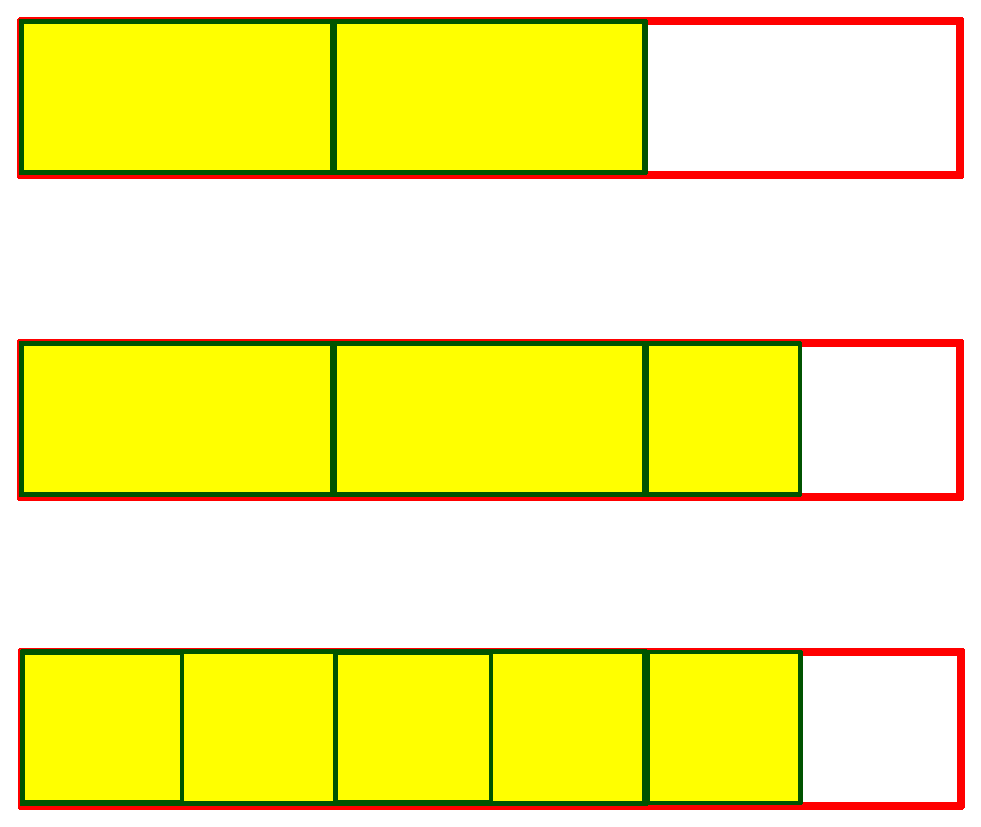
\includegraphics[height=3.5cm, width=6cm]{dibujo-1.eps}};
	    					\node [right] at (8.5, 1.25) {{\Large $\frac{1}{6}$}};
	    					\node [right] at (-.1, 4.6) {Por la mañana vendió $\frac{2}{3}$};
	    					\node [right] at (-.1, 3.25) {Por la tarde vendió la mitad de está en blanco};
	    					\node [right] at (-.1, 1.8) {Dividimos en partes iguales donde cada una es igual a};
	    					\end{tikzpicture}
	    				\end{figure}
	    			\end{minipage}
	    		\end{figure}
    		    \noindent Como vemos en el últmo gráfico, lo vendido a la tarde representa $\frac{1}{6}$.
    		     
	    		\item Si son $2$ periódicos los que no se han vendido, ¿cuántos había al empezar la venta?
	    		\begin{figure}[H]
	    			\begin{minipage}[b]{0.3\textwidth}
	    				Teniendo en cuenta lo realizado en el ítem anterior, observemos que por la tarde le sobraron dos periódicos. Con lo cual, la parte que no está pintada representa a dos periódicos.
	    				
	    				Como vemos en el último gráfico, si sumamos todas las partes no da un total de $12$ periódicos.
	    			\end{minipage}
	    			\hfill \begin{minipage}[b]{0.65\textwidth}
	    				\begin{figure}[H]
	    					\centering
	    					\begin{tikzpicture}
	    					\draw[gris, fill = gris] (0,0) rectangle (10, 5);
	    					\draw[ultra thick, caribbeangreen] (0,0) -- (10, 0) -- (10,5) -- (0, 5)-- (0,0);
	    					\draw[bole, fill = bole] (0,0) rectangle (10, -0.2);
	    					\node at (3.5, 2.6) {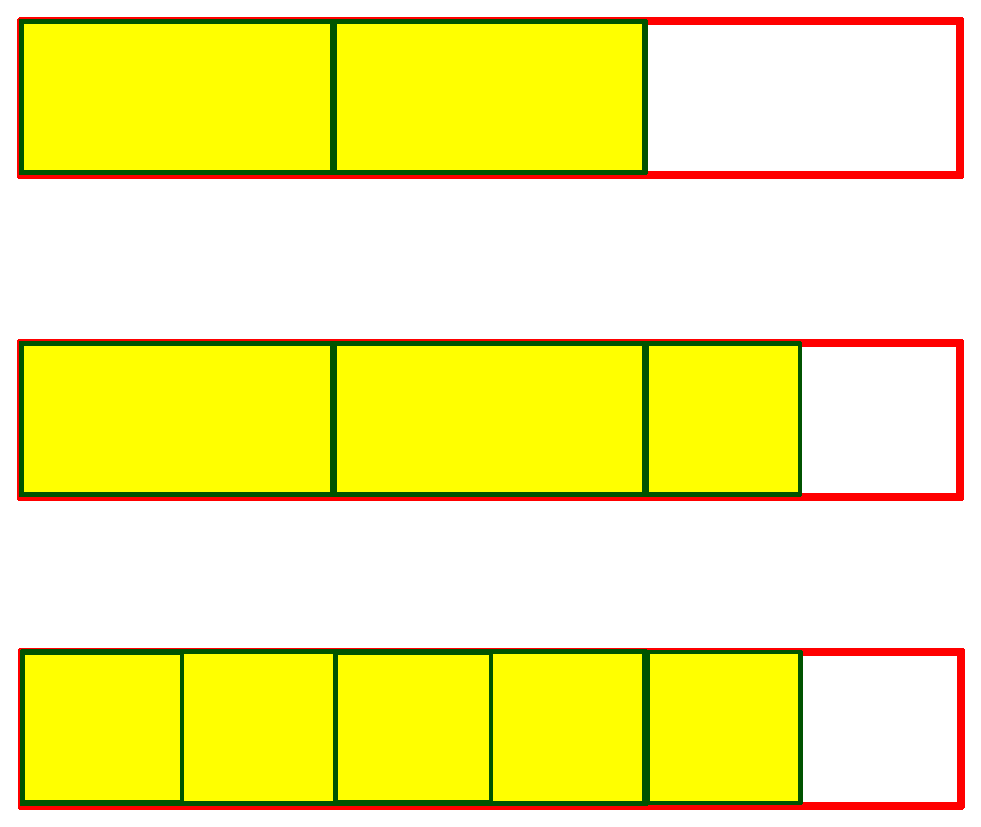
\includegraphics[height=3.5cm, width=6cm]{dibujo-1.eps}};
	    					\node [right] at (-.1, 4.6) {Por la mañana vendió $\frac{2}{3}$};
	    					\node [right] at (-.1, 3.25) {Por la tarde, vuelve a vender pero le quedan $2$};
	    					\node [right] at (-.1, 1.8) {Nos dice que lo que sobró es igual a $2$};
	    					\node [right] at (0.75, 1.25) {$2$};
	    					\node [right] at (1.75, 1.25) {$2$};
	    					\node [right] at (2.75, 1.25) {$2$};
	    					\node [right] at (3.75, 1.25) {$2$};
	    					\node [right] at (4.75, 1.25) {$2$};
	    					\node [right] at (5.75, 1.25) {$2$};
	    					%\node [right] at (5.75, 2.5) {$2$};
	    					\end{tikzpicture}
	    				\end{figure}
	    			\end{minipage}
	    		\end{figure}
	    	\end{enumerate}
	    	\begin{answer}
	    		contenidos de tu respuesta.
	    	\end{answer}
	    \end{question}
        
        \begin{question}
        	Un recipiente está lleno de agua hasta los $\displaystyle{\frac{4}{5}}$ de su capacidad. Se saca la mitad del agua que contiene.
        	
        	\begin{enumerate}
        		\item ¿Qué fracción de la capacidad del recipiente se ha sacado?
        		
        		\hrulefill
        		
        		\item Si la capacidad del recipiente es de $80$ litros, ¿cuántos litros queden en el mismo?
        		
        		\hrulefill.
        	\end{enumerate}
        	\begin{answer}
        		contenidos de tu respuesta.
        	\end{answer}
        \end{question}
	\end{shortanswer}
    %--------------------------------------------------------------------------------------------%
	\begin{endmatter}
		\centerline{\LARGE \textcolor{upforestgreen}{\textbf{Suma de Fracciones de Distinto Denominador:}}}
		\vspace{.4cm}
		\begin{tcolorbox}[colback=red!10!white, colframe=tealgreen, title=\textit{Para pensar!...}]
			\begin{enumerate}%
				\item Leer y analizar la siguiente situación. Luego, resuelvan con el compañero de al lado para seleccionar la respuesta correcta y justifiquen su selección.
				\begin{center}%
					\textit{``Ya pinté $2/3$ del paredón de color amarillo y $1/4$ de color verde. ¿Qué fracción total del paredon está pintado?''...}
				\end{center}%
			\end{enumerate}%
			%$\bullet$
		\end{tcolorbox}
		
		En la situación problemática, tenemos que las fracciones involucradas son $2/3$ y $1/4$ y no poseen el mismo denominador. Por lo tanto, no podemos sumar directamente los numeradores y mantener algún denominador.
		
		Para sumar de fracciones de distinto denomindador debemos hacer que los denominadores de las fracciones involucradas sean iguales realizando el siguiente procedimiento:
		
		\begin{figure}[!h]
			% 30% de la página
			\begin{minipage}[b]{0.3\textwidth}
				Para sumar de fracciones de distinto denomindador debemos hacer que los denominadores de las fracciones involucradas sean iguales, para ello usamos \textit{fracciones equivalentes} para igualarlos, y así nos quedaás fracciones con el mismo denominador
			\end{minipage}
			\hfill \begin{minipage}[b]{0.65\textwidth}
				\begin{figure}[H]
					\centering
					\begin{tikzpicture}
					\draw[gris, fill = gris] (0,0) rectangle (10, 5);
					\draw[ultra thick, caribbeangreen] (0,0) -- (10, 0) -- (10,5) -- (0, 5)-- (0,0);
					\draw[bole, fill = bole] (0,0) rectangle (10, -0.2);
					\node at (3.5, 2.5) {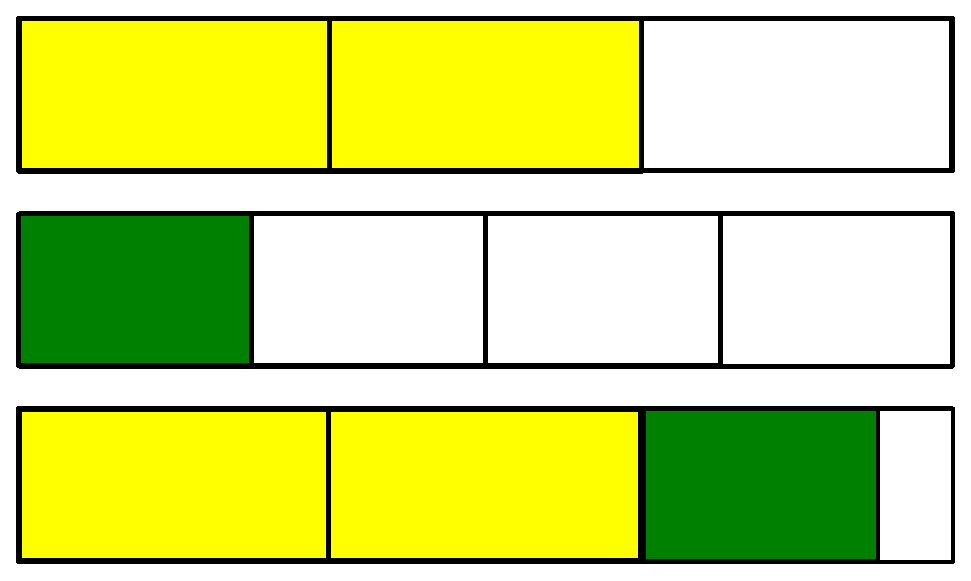
\includegraphics[height=3.5cm, width=6cm]{ActiDesa.eps}};
					\node [right] at (6.5, 3.75) {{\LARGE $\frac{2}{3}$}};
					\node [right] at (6.5, 2.5) {{\LARGE $\frac{1}{4}$}};
					\node [right] at (6.5, 1.25) {{\LARGE $\frac{2}{3}+\frac{1}{4}={\color{red}{\textbf{?}}}$}};
					\draw[blue] (6.81,1) circle [radius = 0.2];
					\draw[blue] (8,1) circle [radius = 0.2];
					\draw[red, ultra thick] (9.25, 1.3) circle [radius = 0.35];
					\end{tikzpicture}
				\end{figure}
			\end{minipage}
		\end{figure}
		\vspace{.4cm}
		\begin{enumerate}
			\item Multiplicamos los denominadores en una tabla como la que se muestra
			
			\begin{center}
				\begin{tabular}{ | c | c | c | c | c | c | }\hline
					\textbf{Denominadores}& $1$ & $2$ & $3$  &          $4$                 & $5$  \\ \hline
					$\textbf{3}$          & $3$ & $6$ & $9$  & ${\color{red}{\textbf{12}}}$ & $15$ \\ \hline
					$\textbf{4}$          & $4$ & $4$ & ${\color{red}{\textbf{12}}}$ & $16$ & $20$ \\ \hline
				\end{tabular}
			\end{center} 
			
			Con esto hallamos el primer resultado en comun de la tabla. Observemos que el primer resultado en común es el número ${\color{red}{\textbf{12}}}$.
			
			\item Identificamos los numeros que vamos a usar para multiplicar ambos denominadores y que de por resultado un valor en común, en este caso, para obtener como resultado ${\color{red}{\textbf{12}}}$. Por ejemplo,  $3\times 4 = {\color{red}{\textbf{12}}}$ y $4\times 3 = {\color{red}{\textbf{12}}}$.
			
			\item Multiplicamos numerador y denominador en ambas fracciones por el numero que de resultado el valor común, es decir, que de como resultado ${\color{red}{\textbf{12}}}$.
			En este ejemplo será
			\begin{align*}
			    \frac{2}{3}&=\frac{2\times 4}{3\times 4}=\frac{8}{{\color{red}{\textbf{12}}}}&&y&\frac{1}{4}&=\frac{1\times 3}{4\times 3}=\frac{3}{{\color{red}{\textbf{12}}}}
			\end{align*}
			
			
			\item Por último.... 
			
			
			\begin{figure}[H]
				\begin{minipage}[b]{0.3\textwidth}
					Obtenemos fracciones equivalentes que poseen el mismo denominador y realizamos \textbf{la suma de fracciones con igual denominador} (procedimiento que se rememoró en la recuperación de saberes previos) de esta manera
					\begin{align*}
					\frac{8}{{\color{red}{\textbf{12}}}}+\frac{3}{{\color{red}{\textbf{12}}}}=\frac{8+3}{{\color{red}{\textbf{12}}}}=\frac{11}{{\color{red}{\textbf{12}}}}  
					\end{align*}
				\end{minipage}
				\hfill \begin{minipage}[b]{0.65\textwidth}
					\begin{figure}[H]
						\centering
						\begin{tikzpicture}
						\draw[gris, fill = gris] (0,0) rectangle (10, 5);
						\draw[ultra thick, caribbeangreen] (0,0) -- (10, 0) -- (10,5) -- (0, 5)-- (0,0);
						\draw[bole, fill = bole] (0,0) rectangle (10, -0.2);
						\node at (3.5, 2.5) {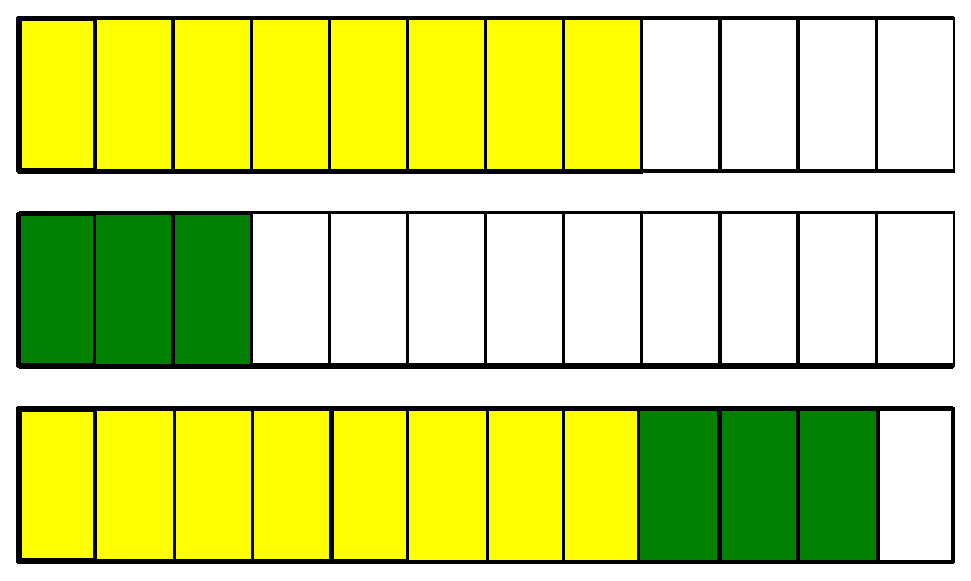
\includegraphics[height=3.5cm, width=6cm]{Actividaddesarrollotres.eps}};
						\node [right] at (6.5, 3.75) {{\Large $\frac{8}{{\color{red}{\textbf{12}}}}$}};
						\node [right] at (6.5, 2.5) {{\Large $\frac{3}{{\color{red}{\textbf{12}}}}$}};
						\node [right] at (6.5, 1.25) {{\Large $\frac{8}{{\color{red}{\textbf{12}}}}+\frac{3}{{\color{red}{\textbf{12}}}}=\frac{11}{{\color{red}{\textbf{12}}}}$}};
						\end{tikzpicture}
					\end{figure}
				\end{minipage}
			\end{figure}     
		\end{enumerate}
	
		\begin{tcolorbox}[colback=red!10!white, colframe=tealgreen, title=\textit{Para pensar!...}:]
			\def\blank#1{$\underline{\mbox{\hphantom{#1}}}$}
			\begin{enumerate}%
				\item Leer y analizar la siguiente situación. Luego, resuelvan con el compañero de al lado para seleccionar la respuesta correcta y justifiquen su selección.
				\begin{center}%
					\textit{``Ya pinté $2/3$ del paredón de color amarillo y $1/4$ de color verde. ¿Qué fracción total del paredon está pintado?''...}
				\end{center}%
				\textbf{Respuesta:}
				\begin{center}
					$\bullet$ ``\textit{Si a $\frac{2}{3}$ le sumamos $\frac{1}{4}$ se tiene que la Fracción total del paredon que  está pintado es \blank{$\frac{8}{12} + \frac{3}{12}= \frac{11}{12}$}}''.
				\end{center}
			\end{enumerate}%
		\end{tcolorbox}
	    %-------------------------------------------------------------------------------------------%
	\end{endmatter}
\end{document}